\documentclass[11pt]{report} % use larger type; default would be 10pt

\usepackage[utf8]{inputenc} % set input encoding (not needed with XeLaTeX)


%%% PAGE DIMENSIONS
\usepackage{geometry} % to change the page dimensions
\geometry{letterpaper} % or letterpaper (US) or a5paper or....
\geometry{margin=0.75in} % for example, change the margins to 2 inches all round
% \geometry{landscape} % set up the page for landscape
%   read geometry.pdf for detailed page layout information

%%% PACKAGES
\usepackage{datetime} % for date without day
\usepackage{graphicx} % support the \includegraphics command and options
\usepackage{epstopdf}
\usepackage{amsmath,amssymb,amsthm}
\usepackage{mathrsfs}                      % Gives us \mathscr for \setset
\usepackage{wrapfig}
\usepackage{array}
\usepackage[table]{xcolor}
\usepackage{booktabs}
\usepackage{titlesec}
\usepackage[normalem]{ulem}
\newcommand{\subfigureautorefname}{\figureautorefname}
\usepackage{chemarr}
\definecolor{Gray}{gray}{0.85}
\newdateformat{monthyeardate}{\monthname[\THEMONTH], \THEYEAR} % new date format
\newcommand{\ra}[1]{\renewcommand{\arraystretch}{#1}}
\newcolumntype{L}[1]{>{\raggedright\let\newline\\\arraybackslash\hspace{0pt}}m{#1}}
\newcolumntype{C}[1]{>{\centering\let\newline\\\arraybackslash\hspace{0pt}}m{#1}}
\newcolumntype{R}[1]{>{\raggedleft\let\newline\\\arraybackslash\hspace{0pt}}m{#1}}
\usepackage{indentfirst}
\usepackage[hidelinks]{hyperref}
\hypersetup{
	colorlinks,
	linkcolor={blue!50!black},
	citecolor={blue!50!black},
	urlcolor={blue!80!black}
}
% for writing algorithms
\usepackage{algpseudocode}
\usepackage{algorithm}

\makeatletter
\newcommand{\removelatexerror}{\let\@latex@error\@gobble}
\makeatother

\usepackage{booktabs} % for much better looking tables
\usepackage{array} % for better arrays (eg matrices) in maths
\usepackage{paralist} % very flexible & customisable lists (eg. enumerate/itemize, etc.)
\usepackage{verbatim} % adds environment for commenting out blocks of text & for better verbatim
\usepackage{subfig} % make it possible to include more than one captioned figure/table in a single float
% These packages are all incorporated in the memoir class to one degree or another...

%%% HEADERS & FOOTERS
\usepackage{fancyhdr} % This should be set AFTER setting up the page geometry
\pagestyle{fancy} % options: empty , plain , fancy
\renewcommand{\headrulewidth}{0pt} % customise the layout...
\lhead{}\chead{}\rhead{}
\lfoot{}\cfoot{\thepage}\rfoot{}

%%% SECTION TITLE APPEARANCE
\usepackage{sectsty}
%\allsectionsfont{\sffamily\mdseries\upshape} % (See the fntguide.pdf for font help)
% (This matches ConTeXt defaults)


%%% ToC (table of contents) APPEARANCE
\usepackage[nottoc,notlof,notlot]{tocbibind} % Put the bibliography in the ToC
\usepackage[titles,subfigure]{tocloft} % Alter the style of the Table of Contents
\renewcommand{\cftsecfont}{\rmfamily\mdseries\upshape}
\renewcommand{\cftsecpagefont}{\rmfamily\mdseries\upshape} % No bold!

%%% New commands%%%%%
\setcounter{secnumdepth}{4}
\titleformat{\paragraph}
{\normalfont\normalsize\bfseries}{\theparagraph}{1em}{}
\titlespacing*{\paragraph}
{0pt}{3.25ex plus 1ex minus .2ex}{1.5ex plus .2ex}

\addtocontents{loa}{\def\string\figurename{Algorithm}} % list of algorithms



%%% GRAPHICS PATH
%\graphicspath{{E:/DissertationProspectus/figures/}}

%%% END Article customizations

%%% The "real" document content comes below...

\begin{document}
	
	%Title Page
	\thispagestyle{empty}
	\begin{center}
		\begin{minipage}{\linewidth}
			\centering
			%Thesis Title
			\vspace{2cm}
			{\Huge \bf{Voice Command Browsing (Extension for Google Chrome  Browser)}\par}
			\vspace{1cm}
			%Report type		
			{\Large \bfseries{MINI PROJECT REPORT}\par}
			\vspace{0.5cm}
			{\Large \emph{Submitted in partial fulfillment of the requirements for the award of degree}\par}
			\vspace{0.5cm}
			{\Large \bf{BACHELOR OF TECHNOLOGY} \par}
			\vspace{0.5cm}
			{\Large \bf{BY} \par}
			\vspace{1cm}
			%Author's name
			{\Large \bf{RAJESH R NAIR}\hspace{3cm}     Reg.no:14015695 \par}
			{\Large \bf{UNNIKRISHNAN}\hspace{3cm}      Reg.no:14015695 \par}
			\vspace{1cm}
			% logo							
			
\includegraphics[width=0.5\linewidth]{figures/logo.png}
			
			%School
			{\Large \bfseries{SCMS SCHOOL OF ENGINEERING AND TECHNOLOGY}\par}
			{\Large \emph{(Affiliated to M.G. University)}\par}
			{\Large VIDYA NAGAR, PALISSERY, KARUKUTTY\par}
			{\Large ERNAKULAM – 683 582\par}
			\vspace{1cm}
			
			%\vspace{2cm}
			
			%Date
			{\Large \monthyeardate \today}
		\end{minipage}
	\end{center}
	\clearpage
	
	
	% Certificate page
	\thispagestyle{empty}
	\begin{center}
		\begin{minipage}{\linewidth}
			\centering
			%\vspace{1cm}			
			% logo					
			
\includegraphics[width=0.5\linewidth]{figures/logo.png}
			\vspace{1cm}
			%School
			\\
			
			{\Large \bf{SCMS SCHOOL OF ENGINEERING AND TECHNOLOGY}\par}
			{\Large \emph{(Affiliated to M.G. University)}\par}
			{\Large VIDYA NAGAR, PALISSERY, KARUKUTTY\par}
			{\Large ERNAKULAM – 683 582\par}
			\vspace{1cm}
			{\Large \bf{\underline{BONAFIDE CERTIFICATE}}\par}
			\vspace{0.5cm}
			\begin{flushleft}
				This is to certify that the mini project, titled ''Voice Command Browsing (Extension for Google Chrome  Browser)'' by
			\end{flushleft} 
			%\vspace{0.5cm}
			%Author's name
			{ \bf{RAJESH R NAIR}\hspace{3cm}     Reg.no:14015695 \par}
			{ \bf{UNNIKRISHNAN}\hspace{3cm}      Reg.no:14015695 \par}
			\begin{flushleft}
				submitted in partial fulfilment of the requirement for the award of the degree of Bachelor of Technology, is a bonafide work carried under supervision, during the academic year 2015-2016.
			\end{flushleft}
			{ \bf{Ms. DEEPA SREE VARMA}\hspace{3.5cm}     Prof. VINOD P \par}
			{ \bf{PROJECT GUIDE}\hspace{3cm}      HEAD OF DEPARTMENT\par}
			
			\vspace{3cm}
			
			{ \bf{INTERNAL EXAMINER}\hspace{3cm}     EXTERNAL EXAMINER \par}
			
			
		\end{minipage}
	\end{center}
	\clearpage
	
	
	
	
	%Abstract Page
	\thispagestyle{empty}
	\begin{center}
		\begin{minipage}{\linewidth}
			\vspace{3cm}
			{\centering \bf{Abstract}\par}
			\vspace{0.5cm}
			Put Abstract here.....
		\end{minipage}
	\end{center}
	\clearpage
	
	
	%ACKOWLEDGEMENT Page
	\thispagestyle{empty}
	\begin{center}
		\begin{minipage}{\linewidth}
			\vspace{3cm}
			{\centering \bf{ACKOWLEDGEMENT}\par}
			\vspace{0.5cm}
			We are greatly indebted to Prof.M.Madhavan, Principal, SSET, Ernakulam and Prof.Vinod, Head of department, Department of Computer Science and Engineering, SSET, who whole heartedly granted us the permission to carry out the mini project.
			We would like to thank our guide, Ms.Deepa Sree Varma, Assistant Professor, Department of  Computer Science and Engineering, SSET who has given us valuable guidance and support throughout the project. Also, we would like to thank our project coordinators, Ms.Shilpa  P C and Ms.Gayathri  Assistant Professors, Department of Computer Science and Engineering, SSET, who supported and instructed us all the way.
			We would like to express our sincere gratitude to all the teachers of Computer Science Department who gave us moral and technical support through the course of our mini project. We would like to thank the supporting staff in the Computer lab whose dedicated work kept the lab working smoothly, thus ensuring our time at the lab went hassle free.
			
		\end{minipage}
	\end{center}
	\clearpage
	
	\tableofcontents
	\listoffigures
	\listoftables
	\newpage

\chapter{Introduction}
\label{chap:Intro}



\section{OVERVIEW}
\label{sec:OVERVIEW}



\section{PROBLEM ANALYSIS}
\label{sec:PROBLEM ANALYSIS}

Problem analysis is the process of understanding the actual problems, user needs and proposing solutions to meet those needs. The goal of problem analysis is to gain a better understanding of the problem being solved before development begins. It is the process of gathering and interpreting facts, diagnosing problems and using the information to recommend improvements on the system. Problem analysis is problem solving activities that require intensive communication between users and the system developers. A problem can be defined as the difference between things as perceived and things as desired. The system is studied and analyzed. The system is viewed as a whole and the input to the system are identified. The output from the system is given to various processes.


\section{EXISTING SYSTEM}
\label{sec:EXISTING SYSTEM}



\section{PROPOSED SYSTEM}
\label{sec:PROPOSED SYSTEM}


\section{FEASIBILITY STUDY}
\label{sec:FEASIBILITY STUDY}

Feasibility study is a procedure that identifies, describes and evaluates candidate systems and selects the best system for the job. An estimate is made whether the identified users need may be satisfied using the current software and hardware technologies. The study will decide whether the proposed system will be cost effective from a business point of view and if it can be developed using the given existing budgetary constraints. 
The key considerations involved in the feasibility analysis are the following:


\begin{enumerate}
	\item Economic feasibility
	\item Technical feasibility
	\item Operational feasibility
\end{enumerate}


\subsection{ECONOMIC FEASIBILITY}
\label{subsec:ECONOMIC FEASIBILITY}

Economic study is the most frequently used method for evaluating the effectiveness of candidate system. More commonly known as cost/benefit analysis, the procedure is to determine the benefits and savings that are accepted from a candidate system and compares with costs. If benefit outweighs cost, then decisions are made to design and implement the system. Otherwise further alterations will have to be made if to have a chance of being approved.
Less hardware is required and can also be mounted on the existing wheelchair with reduced complexity.Hence this project is economically feasible and is cost effective because of its compatibility and effort saving nature.


\subsection{TECHNICAL FEASIBILITY}
\label{subsec:TECHNICAL FEASIBILITY}

Technical feasibility is a measure of how feasible the project is technically. The effort and technology included in the conventional system is not needed as the whole process is automated.
The hierarchy of the new system is very easier than the existing system. The new system is very much easier and user friendly. Operational cost is very easy. The maintenance and modification of the new system needs very less human effort. 

\chapter{DESIGN}
\label{cha:DESIGN}

\section{BLOCK DIAGRAM}
\label{sec:BLOCK DIAGRAM}

\section{BLOCK DIAGRAM}
\label{sec:DATA FLOW DIAGRAMS}

\subsection{CONTEXT LEVEL DFD}
\label{subsec:CONTEXT LEVEL DFD}

\begin{figure}[h]
	\centering
	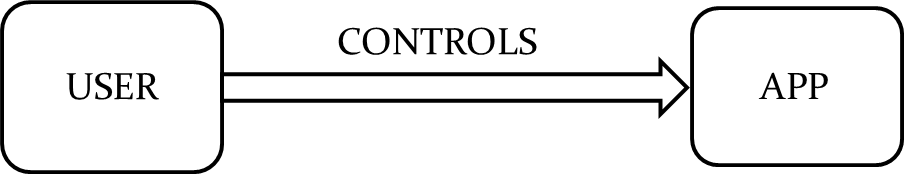
\includegraphics[width=0.5\linewidth]{figures/context_level_DFD.png}
	\caption{Context level DFD}
	\label{fig:Context level DFD}
\end{figure}


\begin{enumerate}
	\item Context level DFD is the most basic representation of the system.
	\item This indicates the basic working of the system.
	\item The user controls the application.
\end{enumerate}


\subsection{LEVEL 0 DFD}
\label{subsec:LEVEL 0 DFD}


\begin{enumerate}
	\item Level 0 DFD indicates the basic processes involved in the system.
	\item This level indicates all the processes of our system.
\end{enumerate}

\subsection{LEVEL 1 DFD}
\label{subsec:LEVEL 1 DFD}

\begin{enumerate}
	\item Level 1 DFD represents the reading of the items by the rfid sensor and its processing.
	\item User can add and remove item to/from the trolley.
\end{enumerate}

\subsection{LEVEL 2 DFD}
\label{subsec:LEVEL 2 DFD}


\begin{enumerate}
	\item Level 2 represents the processing in mobile app and total display.
\end{enumerate}

\section{TABLE}
\label{sec:TABLE}

\subsection{ITEMS}
\label{subsec:ITEMS}


\chapter{IMPLEMENTATION}

\section{SYSTEM REQUIREMENTS}
\label{sec:SYSTEM REQUIREMENTS}


\subsection{HARDWARE REQUIREMENTS}
\label{subsec:HARDWARE REQUIREMENTS}


\subsection{SOFTWARE REQUIREMENTS}
\label{subsec:SOFTWARE REQUIREMENTS}

\section{PLATFORM AND IDE}
\label{sec:PLATFORM AND IDE}


\subsection{ANDROID STUDIO}
\label{subsec:ANDROID STUDIO}


\subsection{ARDUINO IDE}
\label{subsec:ARDUINO IDE}

\section{DETAILS OF IMPLEMENTATION}
\label{sec:DETAILS OF IMPLEMENTATION}

The main objective of our project is to design a wheelchair that will be controlled wirelessly and will be very easy to operate it with no physical efforts.Implementation is the stage of the project when the theoretical design is turned out into a working system. Thus it can be considered to be the most critical stage in achieving a successful new system and in giving the user, confidence that the new system will work and be effective.
The implementation stage involves careful planning, investigation of the existing system and it's constraints on implementation, designing of methods to achieve changeover and evaluation of changeover methods.

\subsection{FUNCTIONAL MODULES}
\label{subsec:FUNCTIONAL MODULES}

The system is divided into 2 modules:

\begin{enumerate}
	\item Hardware module
	\item Application module
\end{enumerate}

\subsubsection{HARDWARE MODULE}
\label{subsubsec:HARDWARE MODULE}

APPLICATION MODULE:

Source code :

\chapter{TESTING}
\label{cha:TESTING}

Testing is the most important activity in the development phase. Testing is the process of    finding   errors or bugs in the system. Testing ensuresthe satisfaction of the users. In other words it isprocess by which one detects the defects in the system. Software testing methods are  traditionally divided into black box testing and white box testing. These two approaches are used to describe the point of view that a test engineer takes when designing test cases.

\section{TEST PLANS}
\label{sec:TEST PLANS}

The implementation of a computer-based system requires that test data can be prepared and that the system and its elements be tested in a planned, structured manner. The computer program component is a major subsystem of the computer-based information system, and particular attention should be given to the testing of these system elements as it is developed.
Testing is a process of executing a program with the interest of finding an error. A good test is one that has a high probability of finding the yet undiscovered errors. The primary objective for the test case design is to drive a set of tests that has the highest likelihood for systematically uncovering different classes of errors in the software. A series of testing are performed for this project before the system is ready for acceptance.  Some of the testing strategies applied for the system are listed here.

Testing Strategies: 
\begin{enumerate}
	\item Black Box Testing
	\item White Box Testing
\end{enumerate}

\subsection{Black Box Testing}
\label{subsec:Black Box Testing}

Black Box testing also called functional testing, focuses on the functional requirements of the software. Knowing the specified function that a product designed to perform the test can be conducted to ensure that each function is fully operational. Black Box tests are carried out to test that input to function is properly accepted and output is correctly produced. It finds the errors in the following categories:

\begin{enumerate}
	\item Interface errors.
	\item Performance in data structures or external database access.
	\item Performance errors.
	\item Initialization and termination errors.
	\item Incorrect or missing functions.
\end{enumerate}

Black box testing is used to detect errors of type incorrect or missing functions, interface errors, errors in data structures or external database access, performance, initialization and termination errors. 

\subsection{White Box Testing}
\label{subsec:White Box Testing}

White box testing, sometimes called -- Glass box testing, and is a test case design uses the control structure of the procedural design to check the errors. It involves following procedures: 

\begin{enumerate}
	\item All independent paths within module have been exercised at least once.
	\item All logical decisions were checked for the true and false values.
	\item All loops were executed to check their boundary values. 
	\item Internal data structure was tested for their validity. 
\end{enumerate}


\subsection{TYPES OF TESTING}
\label{subsec:TYPES OF TESTING}

\begin{enumerate}
	\item Unit Testing 
	\item Integration Testing
	\item Validation Testing 
	\item Output Testing 
	\item User Acceptance Testing 
	\item Product transitions qualities 
\end{enumerate}

\section{TESTCASE TABLES}
\label{sec:TESTCASE TABLES}

\begin{table}[h]
	\centering
	\caption{CONNECTION PAGE}
	\label{tab:CONNECTION PAGE}
	\begin{tabular}{|l|l|l|}
		\hline
		\textbf{SL NO.} & \textbf{TEST CASE} & \textbf{RESULT} \\ \hline
		\textbf{1}      & \textbf{}          & \textbf{}       \\ \hline
		\textbf{2}      & \textbf{}          & \textbf{}       \\ \hline
		\textbf{3}      & \textbf{}          & \textbf{}       \\ \hline
	\end{tabular}
\end{table}


\chapter{RESULTS AND DISCUSSIONS}

\section{PROBLEMS FACED}

\section{SYSTEM ACHIEVEMENTS}


\chapter{CONCLUSION AND FUTURE SCOPE}


\chapter{APPENDIX}


\section{SCREEN SHOTS} 
\label{App:Appendix1}

\subsection{HOME PAGE}



\begin{appendix}    
	
\end{appendix}

%\nocite{Charaka}
%\nocite{Ayurvedic}
%\nocite{Susrutha}
%\nocite{Chikitsa}
%\nocite{Shodala}
%\nocite{Arka}
%\bibliographystyle{unsrt}
%\bibliography{synopsis}

\end{document}